\chapter{Background}
\label{background}
In this chapter the technologies that form the foundation of Dynamic OpenCL are explained. Additionally, several competing solutions are considered for further insight into the decision process that considers arguments in favor or against a specific approach.

\section{Basic Distribution Methods}
\label{distribution_basics}

\subsection*{OpenMP and OpenACC}
OpenMP represents a compiler extension that allows programmers to harness parallel computational power on a machine. It adds functions and flags to the respective language (C, C++ and Fortran are currently supported), which instruct the execution environment how to parallelize the program \cite{openmp_spec}. The resulting code can then be run in multiple threads that can be scheduled on many CPU cores in parallel. OpenACC offers similar functionality as OpenMP but aims at offloading parallel computations to attached accelerators like GPUs \cite{openacc_spec}. Thus if offers additional keywords specifically for assigning parallel computations to available accelerators.

\begin{lstlisting}[caption=OpenMP Code Example in C,captionpos=b,label=lst:openmp_code]
void example()
{
  int i;
  int n = 10;
  #pragma omp parallel for
  for (i=0; i<n; i++)
    printf("%d", i);
}
\end{lstlisting}

The OpenMP example in Source Code \ref{lst:openmp_code} presents a simple parallelized loop that prints the index of the current iteration. As multiple iterations can be executed at the same time, the printed digits do not necessarily have to be in order.

\subsection*{MPI}
Although OpenMP and OpenACC are powerful tools for parallelization on a single machine, in order to write large scale software, communications across multiple machines are necessary. One standard to enable internode communicaion is MPI. MPI is implemented for multiple languages and extends them with functions to identify a process and send as well as receive messages\cite{mpi_spec}. While the provided mechanisms may be used to run multiple parallel processes on a single machine, they can also be employed to accomplish communications between cluster nodes.

\begin{lstlisting}[caption=MPI Code Example in C,captionpos=b,label=lst:mpi_code]
#include <stdio.h>
#include <string.h>
#include <mpi.h>

int main(int argc, char **argv){
  char messageBuffer[64];
  int rank, processCount;

  MPI_Init(&argc, &argv);
  MPI_Comm_rank(MPI_COMM_WORLD, &rank);
  MPI_Comm_size(MPI_COMM_WORLD, &processCount);

  if(rank == 0){
    for(int i = 1; i<processCount;i++){
      sprintf(messageBuffer, "This is a message from Process 0.");
      MPI_Send(messageBuffer, sizeof(messageBuffer), MPI_CHAR, i, 0, MPI_COMM_WORLD);
    }
  }else{
    MPI_Recv(messageBuffer, sizeof(messageBuffer), MPI_CHAR, 0, 0, MPI_COMM_WORLD, MPI_STATUS_IGNORE);
    printf("Process %d receives: %s\n", rank, messageBuffer);
  }

  MPI_Finalize();
  return 0;
}
\end{lstlisting}

MPI programs can be run with a specified number of processes. Executing Source Code \ref{lst:mpi_code} with 4 processes initiates a simple communication from the first process to all other processes. The given code is executed in every process but each process identifies its own rank, which is used to define whether to send or to receive a message. Running the code may yield the following console output:
\begin{Verbatim}[fontsize=\small]
Process 1 receives: This is a message from Process 0.
Process 3 receives: This is a message from Process 0.
Process 2 receives: This is a message from Process 0.
\end{Verbatim}

\subsection*{MapReduce}
MapReduce is a programming model introduced by Google specifically targeted at processing large amounts of data\cite{mapreduce}. Its most prominent implementation is Hadoop MapReduce, which runs in combination with the Hadoop Distributed File System (abbr. HDFS)\cite{hadoop_mapreduce}. The HDFS is mostly used to store processable files, which represent subdivisions of a large dataset, also called input splits. An input split is handled independently by a so called \textit{Map} function, which executes a given algorithm on the partial dataset and generates an intermediate result for this split. These intermediate results are then passed to a \textit{Reduce} function, which performs aggregations to yield a final result for the overall dataset. MapReduce is therefore well suited for data intense jobs like log analysis. In figure \ref{img:mapreduce_arch} an exemplary overview of the computational process is given for a 10 Terabyte log, which is split into 10,000 smaller files of 1 Gigabyte each. Each file serves as the input for a \textit{Mapper} process that executes the defined \textit{Map} function and sends its intermediate results to a single \textit{Reducer} that writes the final result back to HDFS.

\begin{figure}[!htb]
	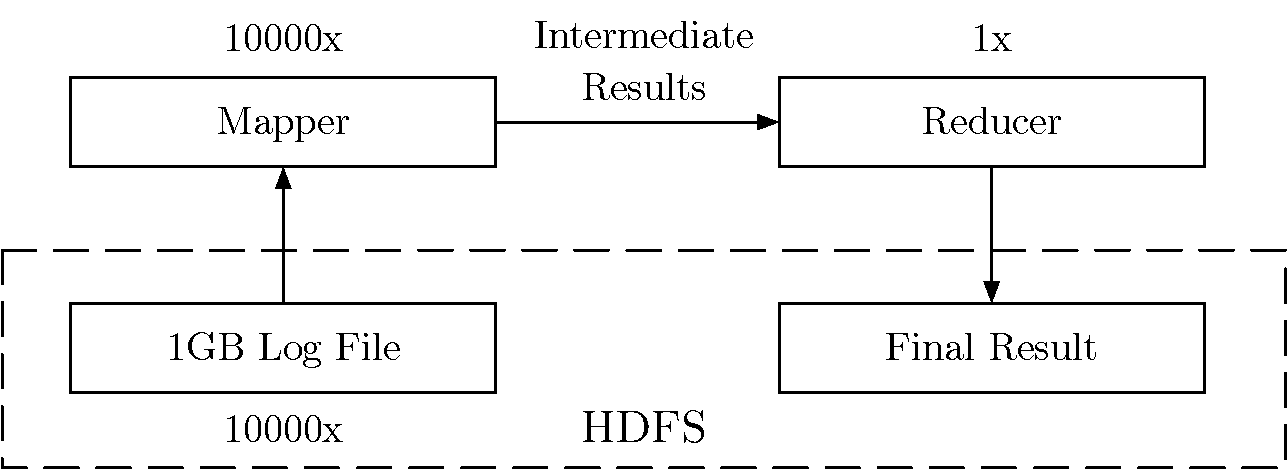
\includegraphics[width=0.75\textwidth]{drawings/mapreduce_arch.pdf}
	\centering
	\caption{MapReduce Example Execution Architecture}
	\label{img:mapreduce_arch}
\end{figure}

\section{OpenCL}
\label{opencl}
OpenCL is a compute framework for supporting parallel programs on heterogeneous hardware. It was initially proposed by Apple but is currently maintained by the Khronos Group, which consists of a multitude of companies like AMD, Intel, NVIDIA and others\cite{opencl_directors}. OpenCL represents a direct competitor to NVIDIA's CUDA computing platform but unlike CUDA is not limited to NVIDIA GPUs. Instead it supports various device types and vendors. In fact OpenCL programs may be executed on CPUs, GPUs, field-programmable gate arrays (abbr. FPGA) and digital signal processors (abbr. DSP). Prerequisite for the execution of OpenCL code on a targeted device is the presence of an OpenCL Installable Client Driver (abbr. ICD) on its enclosing host machine. Such ICDs must conform with the specification released by the Khronos Group. As of today, various implementations of OpenCL exist by vendors like AMD, NVIDIA, Intel, Apple, ARM, Xilinx and others\cite{opencl_conform}.

The most important definitions within the OpenCL specification are the introduction of its execution model as well as the underlying memory model, which in the following are explained based on the OpenCL Specification Version 2.2 document\cite{opencl_spec}.

\subsection*{Execution Model}
OpenCL programs are executed on selected OpenCL devices. An OpenCL program consists of at least one function that is called a Kernel. A Kernel is run for each work-item, which is the smallest partial unit of a submitted task. For instance, a work-item could be an element of an array that is being handled. Kernels process the work-items using so called ranges, which define the size of the overall work-item space in up to three dimensions and allow the Kernel to determine the position of the work-item being processed. Ranges also define how the work-items are subdivided in work-groups. These relations are depicted in figure \ref{img:opencl_data_model} for a two dimensional array that is divided into work-groups in both dimensions.

\begin{figure}[!htb]
	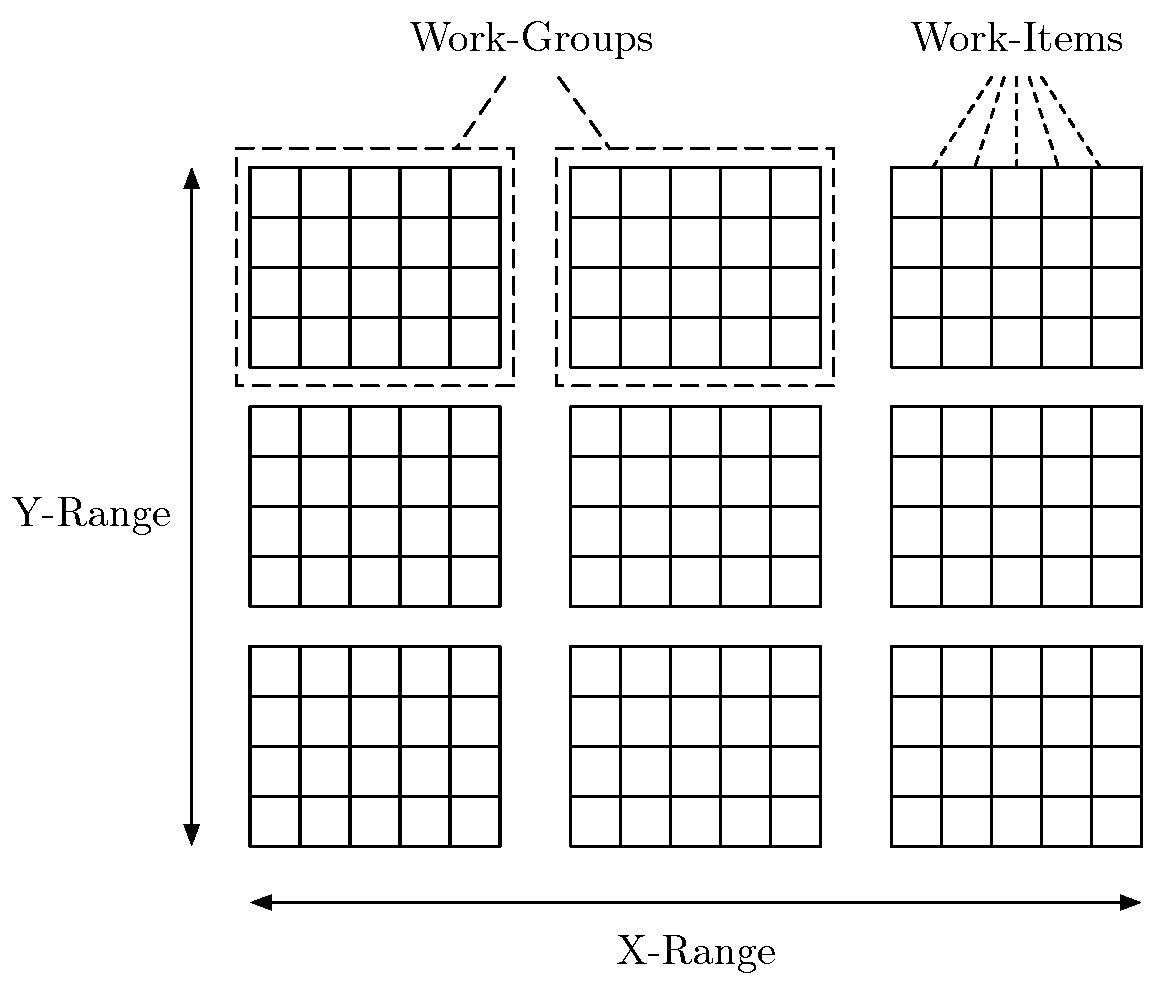
\includegraphics[width=0.55\textwidth]{drawings/opencl_data_model.pdf}
	\centering
	\caption{OpenCL Data Model (adapted from Figure 3-3 in \cite{opencl_spec})}
	\label{img:opencl_data_model}
\end{figure}

In the OpenCL model devices consist of compute units (abbr. CU), which for instance are CPU cores. Each work-group is assigned to a CU that processes it. Through the execution model two layers of parallelization can be applied. Firstly work-groups are independent of each other, allowing their parallel execution when a device has more than one CU installed. Secondly the underlying CUs may be able to parallelize the execution for work-items within a work-group as well. In fact, the parallelization of work-items entirely depends on the respective hardware capabilities and vendor implementation. For example, modern AMD GPUs execute work-groups in so called wavefronts. A wavefront can contain up to 64 work-items, which are executed in batches of 16 items per clock cycle and thus take 4 clock cycles to cover all enclosed items\cite{amd_opencl_spec}. This means that an optimal work-group size for these devices is a multiple of 64 to ensure full utilization of a wavefront.
NVIDIA GPUs on the other hand execute work-groups in so called warps, which can hold up to 32 work-items that are processed in parallel by 32 threads\cite{nvidia_pascal_spec}. This illustrates the level of abstraction of OpenCL, which unifies devices with significantly differing hardware implementations to compute using a single model.

Having many work-groups assigned per CU also enables OpenCL to hide latencies for required memory accesses. Whenever a CU needs to access memory, which would stall its threads, the CU may switch to another processable work-group and continue execution until this work-group also stalls. Thus the time for memory accesses is spent on computations instead of waiting.

\subsection*{Memory Model}

Memory in OpenCL is divided into two major regions, the host memory and the device memory. The host memory is used by the host to store Kernels and execution data. For an execution the required data is transferred from the host memory to the device memory, which is subdivided into different levels:

\begin{description}[align=left,leftmargin=0cm]
  \item [Private] Private memory is only accessible by a single work-item that owns it. As such it is mainly used for temporary variables and allows no sharing to other work-items.
  \item [Local] Local memory is accessible by all work-items within a work-group. Thus it can be used to share and synchronize data within a group. For example, intermediary results for an entire work-group can be produced.
  \item [Global] The global memory can be read and written by the host and all work-items. Therefore it serves to synchronize all work-groups. For instance, the final results of a computation are stored in global memory to be read by the host.
  \item [Constant] Constant memory is similar to global memory but can only be allocated and initialized by the host. Work-items are only allowed to read data, which makes it meaningful for data that does not change throughout the computations.
\end{description}

All of the available memory levels have different sizes, depending on the utilized device and also require a varying number of clock cycles per access. For example, reading data from local memory can be a magnitude faster than from global memory but global memory offers far more space and allows for synchronization among all work-groups. Additionally calls to the global memory may be cached based on the caching capabilities of the respective device.

\subsection*{Kernels}

OpenCL Kernels are written in OpenCL C, which is a superset of C99, containing additional keywords that are related to memory access and synchronization. Kernels have to be started from so called host code, which runs on the machine that contains the targeted devices. The host code is usually written in C or C++ as the standard offers APIs for these languages. Still, third parties offer bindings for other languages. Table \ref{table:opencl_language_bindings} contains some available language bindings.

\begin{table}[htb]
	\centering
	\begin{adjustbox}{width=0.3\textwidth}
		\small
		\begin{tabular}{l | l}
			\textbf{Language}	& \textbf{Bindings}   \\
			\hline
			Java        &  JOCL, Aparapi\\
			.NET        &  OpenCL.NET, Cloo\\
			Python      &  PyOpenCL, PyCL\\
			Ruby	    &  Ruby-OpenCL\\


		\end{tabular}
	\end{adjustbox}

	\caption{OpenCL Language Bindings}
	\label{table:opencl_language_bindings}
\end{table}

\begin{minipage}{\linewidth}

\begin{lstlisting}[caption=OpenCL Vector Addition Kernel,captionpos=b,label={lst:opencl_kernel}]
#pragma OPENCL EXTENSION cl_khr_fp64 : enable

__kernel void run(__global double *a, __global double *b, __global double *c){
  int i = get_global_id(0);
  c[i]  = a[i] + b[i];
}
\end{lstlisting}
\end{minipage}
Source Code \ref{lst:opencl_kernel} presents an OpenCL Kernel that describes the addition of two vectors, in which the elements at identical indexes of two arrays are accumulated. Line 1 enables the OpenCL extension for double-precision floating point numbers, which is necessary for running the code. In line 3 the method declaration is present that consists of three parameters. Each parameter is a pointer to an array of doubles, which reside in \textit{global} memory. As the Kernel is run for every work-item, line 4 identifies the global work-item index by calling \textit{get\_global\_id}. The acquired index is used in line 5 to process the actual computation where the result of the sum of array \textit{a} and array \textit{b} at the corresponding index is written to array \textit{c}.

For this example to run, the host code has to choose an appropriate device, initiate data transfers and perform other auxiliary tasks. The host code is omitted for clarity as with around 50 lines of code it is considerably longer than the actual kernel code.

While the OpenCL standard enables the execution of identical code on heterogeneous platforms, certain limitations still apply based on the capabilities of the utilized devices. For instance, code that uses the double data type can only be successfully run on devices that offer that feature. Executing the above snippet on an \textit{Macbook Air (Early 2015)} may lead to two different results. On the one hand, execution on the built-in \textit{Intel i5-5250U} CPU will correctly add the two provided arrays and return the result. On the other hand the included \textit{Intel Iris Graphics 6100} GPU will produce an error as it does not support the required OpenCL \textit{FP64} extension.

While OpenCL supports more device types and vendors, it seems questionable whether having a general programming model comes with the price of performance penalties when compared to the specialized CUDA platform. \citeauthor{performance_comparison} have shown that CUDA code may be ported to OpenCL with only few modifications but will run between 16\% and 67\% slower depending on the problem size of their implemented Monte Carlo simulation\cite{performance_comparison}. On the opposite \citeauthor{comprehensive_performance_comparison} have come to the conclusion that such performance gaps are influenced by the differences between the programming models and may be prevalent due to programming mistakes and compiler optimizations\cite{comprehensive_performance_comparison}. They reason that with all issues in mind, OpenCL can reach the same performance as CUDA.

\section{Aparapi}
\label{aparapi}
Aparapi is a library that offers extensive functionality to ease the usage of the OpenCL API and minimize programming effort when developing OpenCL Kernels\cite{aparapi}. Firstly, it contains bindings to access OpenCL functions through a Java Native Interface (abbr. JNI), abstracting and bundling multiple low level calls to Java high level functions. Secondly, Aparapi is able to translate Java code to valid OpenCL kernels. An overview of the call chain is given in figure \ref{img:aparapi_call_chain}.

\begin{figure}[!htb]
	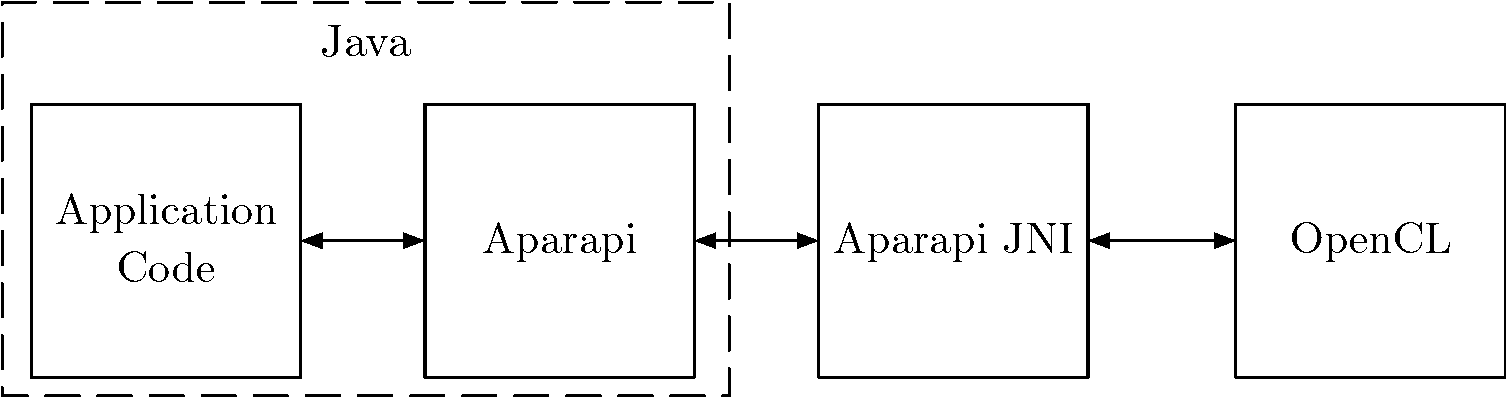
\includegraphics[width=0.75\textwidth]{drawings/aparapi_call_chain.pdf}
	\centering
	\caption{Aparapi Call Chain}
	\label{img:aparapi_call_chain}
\end{figure}

\begin{minipage}{\linewidth}
\begin{lstlisting}[caption=Aparapi Vector Addition Kernel,captionpos=b,label=lst:aparapi_kernel]
final double[] a = new double[]{0, 1, 2, 3, 4, 5, 6, 7, 8, 9};
final double[] b = new double[]{0, 1, 2, 3, 4, 5, 6, 7, 8, 9};
final double[] c = new double[10];

Kernel kernel = new Kernel() {
  @Override
  public void run() {
     int i = getGlobalId();
     c[i] = a[i] + b[i];
  }
};

kernel.execute(10);
System.out.println(Arrays.toString(c));
\end{lstlisting}
\end{minipage}
The Source Code \ref{lst:aparapi_kernel} reproduces the vector addition example code from section \ref{opencl} in which elements at the same index of two arrays are summed and written to a third array. Ultimately, each element from the result array is printed. It also highlights that input data may be defined in Java code itself and the results are again available in Java after execution. This is possible as Aparapi automatically copies the participating data back and forth between the host code and the executing device. For a more granular approach, developers can also define which data should be written or read in order to improve performance. This is especially useful when input data does not change during computation and therefore does not have to be copied back to the host. While an original OpenCL implementation would require roughly 50 lines of auxiliary code, Aparapi hides tasks like device selection and data handling behind its API when no specific control is needed. This enables developers to program algorithms considerably faster and offers beginners a quick access to OpenCL features without knowledge of low level mechanisms.

Although the code translation of Aparapi may work for many use cases, certain limitations apply to the Java code that can be handled. Information about these restrictions can be found in the documentation on GitHub\cite{aparapi_kernel_guidelines}, which is partly outdated as newer features lifted corresponding limitations. In the current version, Aparapi only supports the primitive data types boolean, byte, short, int, long, and float. While programmers may also employ object orientation, Aparapi can only translate classes whose attributes are again primitives. Additionally, not all control-flow features of Java are supported by Aparapi. Indeed it can only handle conditionals and counting \textit{for}-loops. Thus, \textit{switch}, \textit{break}, \textit{continue}, enhanced \textit{for}-loops and recursion are not allowed.
